\chapter{Importing Functional Mock-up Units}
\label{MMFMI}

\section{Setting up a simulation}
\label{sec:setting_up}
The FMI wrapper is started by the StartTLMFMIWrapper startup script.
This script generates the \texttt{tlm.config} file and calls the FMIWrapper executable.
The executable takes the following arguments:\\

\noindent \verb|FMIWrapper <path> <fmufile> <solver> <debug>|\\

Example:\\

\noindent \verb|FMIWrapper C:\temp\folder mymodel.fmu solver=CVODE -d|\\

The last to arguments are optional.
Available solvers are \texttt{Euler}, \texttt{RungeKutta}, \texttt{CVODE} and \texttt{IDA}.
Section \ref{sec:fmi_me} contains more details about the different solvers.
These can currently only be changed by modifying the startup script, i.e. not from the graphical interface.

An FMU keep track of its variables by integer numbers called \texttt{value references}.
However, it does not provide any information about the mapping between its variables and the TLM interface.
Hence, this information must be provided by the user.
A configuration file called \texttt{fmi.config} is used for this purpose, see listing \ref{lst:fmiconfig}.

\lstdefinelanguage{fmiconfig}
{
  % list of keywords
  keywords={
    substeps,
    name
  },
  keywords=[2]{
    position,
    orientation,
    speed,
    ang_speed,
    force
  },
  keywordstyle=\ttfamily\bfseries\textcolor{blue},
  keywordstyle=[2]\ttfamily\bfseries
 % sensitive=false, % keywords are not case-sensitive
 % morecomment=[l]{//}, % l is for line comment
 % morecomment=[s]{/*}{*/}, % s is for start and end delimiter
 % morestring=[b]" % defines that strings are enclosed in double quotes
}

\begin{lstlisting}[language=fmiconfig,basicstyle=\ttfamily,floatplacement=ht,caption=A configuration file maps value references to TLM variables,label=lst:fmiconfig]
substeps,10

name,tlm1
dimensions,6
causality,Bidirectional
domain,Mechanical
position,6,7,8
orientation,136,139,142,137,140,143,138,141,144
speed,9,10,11
ang_speed,145,146,147
force,133,134,135,167,168,169

name,tlm2
dimensions,1
causality,Bidirectional
domain,Mechanical
position,12
speed,15
force,136

name,input1
dimensions,1
causality,Input
domain,Signal
value,16

name,output1
dimensions,1
causality,Output
domain,Signal
value,17
\end{lstlisting}
\newpage
As can be seen, data is stored in a comma-separated format.
The first line specifies the number of substeps used for FMI for Co-Simulation (see section \ref{sec:fmi_cs}).
After this comes the port information.
Each port is specified by name, dimensions, causality and domain, followed by a list of variables depending on the port type.
The numbers after each variable are the value references.
These can be obtained by analyzing the \texttt{modelDescription.xml} file.
Listing \ref{lst:modeldescription} shows an example.
The variable first torque component has the value reference 167.
Hence, this number should be inserted as number four on the "force" line in \texttt{fmi.config}.

\begin{lstlisting}[language=XML,float,floatplacement=ht,caption=Value references for variables are obtained from \texttt{modelDescription.xml},label=lst:modeldescription]
  <ScalarVariable
    name="fMITLMInterface3D1.t[1]"
    valueReference="167"
    variability="continuous"
    causality="local">
    <Real/>
  </ScalarVariable>
\end{lstlisting}


\clearpage
\section{FMI for Co-Simulation}
\label{sec:fmi_cs}
With FMI for Co-Simulation the solver is embedded within the FMU.
Variables can only be exchanged at predefined communication points.
Hence, it is not possible for the solver to obtain interpolated force variables during internal iteration steps.
Keeping the force constant during the entire communication interval may, however, have a negative effect on numerical stability.
For this reason it is possible to divide each communication interval into a fixed number of \textit{sub steps}, as defined in the \texttt{fmi.config}.
In this way the forces can at least be updated in the FMU at more fine-grained intervals.
Pseudo-code for the simulation loop in the wrapper is shown in listing \ref{lst:wrapper_cs}.
The real code also contains error handling, but it has been excluded here to enhance readability.

\lstset{emph={fmu},emphstyle={\color{red}\bfseries},
        emph={[2]TLMPlugin},emphstyle={[2]\color{blue}\bfseries}
}
\begin{lstlisting}[language=c++, basicstyle=\ttfamily\small,floatplacement=htb,caption=Pseudo code for the simulation loop with FMI for co-simulation,label=lst:wrapper_cs]
while (tcur < tend) {
    double hsub = hmax/nSubSteps;
    for(size_t i=0; i<nSubSteps; ++i) {
        x = fmu.get_real(x_vr,3);
        T = fmu.get_real(T_vr,9);
        v = fmu.get_real(v_vr,3);
        w = fmu.get_real(w_vr,3);
        f = TLMPlugin.GetForce(tcur,x,T,v,w);
        fmu.set_real(f_vr[j],6,f);
        
        TLMPlugin.SetMotion(tcur,x,T,v,w);

        fmu.do_step(tcur,hsub);
        tcur+=hsub;

        x = fmu.get_real(x_vr,3);
        T = fmu.get_real(T_vr,9);
        v = fmu.get_real(v_vr,3);
        w = fmu.get_real(w_vr,3);
    }
}
\end{lstlisting}

Note that it is necessary to read the motion variables from the FMU before obtaining the force from the TLMPlugin. 
At the end of each major step it is also necessary to call \texttt{GetForce()} before calling \texttt{SetMotion()}.
The reason for this is that \texttt{SetMotion()} requires updated input variables which are retreived by \texttt{GetForce()}.

\vspace{0cm}

\clearpage
\section{FMI for model exchange}
\label{sec:fmi_me}
With model exchange, the wrapper must provide a solver for the FMU.
Three solvers are available: explicit Euler, 4th order explicit Runge-Kutta, and the CVODE and IDA solvers from Sundials \cite{hindmarsh2005}.
Listing \ref{lst:wrapper_me} shows pseudo code for one major step (i.e. one communication interval) with the IDA solver.
Note that the solver is used with one step mode.
This means that it takes one step at a time, until its internal time exceeds the next communication interval.
The CVODE solver requires a callback function for obtaining derivatives of state variables (i.e. "right-hand side").
The IDA solver requires a similar callback for obtaining the residuals.

\begin{lstlisting}[language=c++, basicstyle=\ttfamily\small,floatplacement=h,caption=Pseudo code for the simulation loop with FMI for model exchange,label=lst:wrapper_me]
double position[3],orientation[9],speed[3],ang_speed[3],force[6];

x = fmu.get_real(x_vr,3);
T = fmu.get_real(T_vr,9);
v = fmu.get_real(v_vr,3);
w = fmu.get_real(w_vr,3);
f = TLMPlugin.GetForce(tcur,x,T,v,w);
fmu.set_real(f_vr[j],6,f);

y = fmu.get_continuous_states();
dy = fmu.get_derivatives();

tcur += h;

while(tc < tcur){
    IDASolve(mem, tcur, &tc, y, dy, IDA_ONE_STEP);
}

fmu.set_continuous_states(y);
\end{lstlisting}

\clearpage
\section{Example: Double Pendulum with Dymola and OpenModelica}
This section will explain how to build a meta model of a double pendulum using FMUs exported from Dymola and OpenModelica.
Figure \ref{fig:double_pendulum} shows a sketch of the model.
The resulting meta model is found in the \texttt{/MetaModels/FmuFmuPendulum} folder.
One FMU for Co-simulation and one for Model Exchange will be used.
Both models use a custom Modelica library called FMILIB for the TLM interfaces.
This library is shipped together with the FMI wrapper.

\begin{figure}[ht]
\centering
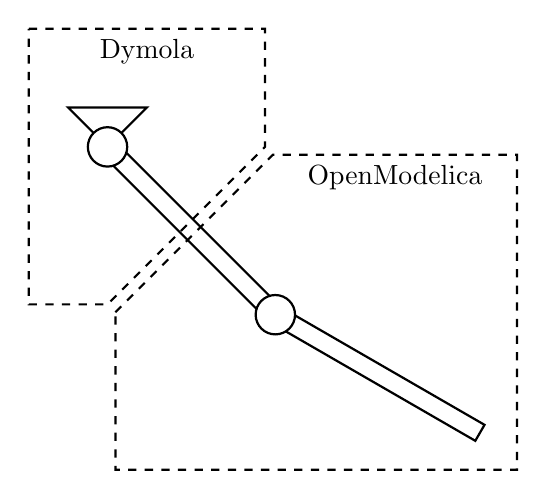
\begin{tikzpicture}
\node[draw,thick,minimum width=3cm,rectangle,rotate=-45,fill=white,xshift=1.5cm] (beam1) {};
\draw[thick,loop] (0,0) -- (0.5cm,0.5cm) -- (-0.5cm,0.5cm) -- (0,0);
\node[draw,thick,circle,minimum width=0.5cm,fill=white] () {};
\node[draw,thick,minimum width=3cm,rectangle,rotate=-30,fill=white,xshift=1.5cm] at(beam1.east) (beam2) {};
\node[draw,thick,circle,minimum width=0.5cm,fill=white] at (beam1.east) () {};

\draw[thick,dashed] (-1cm,1.5cm) -- node[below] () {Dymola} (2cm,1.5cm) -- (2cm,-0.0cm) -- (-0.0cm,-2cm) -- (-1cm,-2cm) -- (-1cm,1.5cm);

\draw[thick,dashed] (0.1cm,-2.1cm) -- (2.1cm,-0.1cm) --node[below] () {OpenModelica} (5.2cm,-0.1cm) -- (5.2cm,-4.1cm) -- (0.1cm,-4.1cm) -- (0.1cm,-2.1cm);
\end{tikzpicture}
\caption{A double pendulum is simulated using FMUs exported from Dymola and OpenModelica}
\label{fig:double_pendulum}
\end{figure}

\subsection{Preparing Dymola FMU of first part pendulum}

The Dymola model consists of half the first pendulum and the fixed attachment to the inertial system, see figure \ref{fig:model_dymola}.
It is normally advisable to decouple a model at its weakest point, which in this case would be at the joint between the two pendulum arms.
In this case the model is decoupled in the middle of the first pendulum only to demonstrate the possibilities.
Force and torque variables must be specified as input variables at the top level of the model, in order to get the correct number of equations and variables.
Hence, we need to add the equations shown in listing \ref{lst:dymola_equations}.

\begin{lstlisting}[language=Modelica,basicstyle=\small\ttfamily, floatplacement=ht,label=lst:dymola_equations,caption=Input variables must be specified on top level in the Modelica models]
  [...]
  //Define FMI interface model
  FMITLM.FMITLM_Interface_3D.FMITLMInterface3D fMITLMInterface3D;
  
  //Define input force and input torque
  input Real f[3](start = zeros(3));
  input Real t[3](start = zeros(3));
equation
  //Assign force and torque in interface model with input variables
  fMITLMInterface3D.f = f;
  fMITLMInterface3D3D.t = t;
  [...]
\end{lstlisting}

\begin{figure}[ht]
\centering
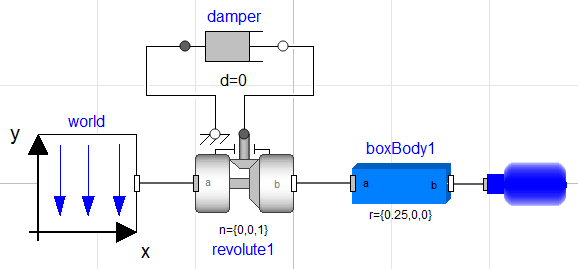
\includegraphics[width=0.65\textwidth]{figs/model_dymola.png}
\caption{The first half of the first beam is modelled in Dymola}
\label{fig:model_dymola}
\end{figure}

Now it is time to export the model so it can be used with the framework.
\begin{enumerate}
\item \textbf{Transform the model to an FMU for co-simulation.}\\
      Use a suitable solver, for example CVODE.
\item \textbf{Put the \texttt{.fmu} file in a new subfolder.}
\item \textbf{Create an empty text file called \texttt{fmi.config} in the same folder.}
\item \textbf{Specify number of substeps on the first line.}\\
              For example: "substeps,10"
\item \textbf{Open \texttt{modelDescription.xml}.}\\
              By opening the \texttt{.fmu} as a zip package.
\item \textbf{Locate the TLM variables and write the value references in \texttt{fmi.config}.}\\
              The desired variables are position, orientation, velocity, angular velocity, force and torque:\\
              \texttt{fMITLMInterface3D.r[x]}, \texttt{fMITLMInterface3D.A[x,y]},\\
              \texttt{fMITLMInterface3D.v[x]}, \texttt{fMITLMInterface3D.w[x]},\\
              \texttt{fMITLMInterface3D.f[x]}, \texttt{fMITLMInterface3D.t[x]}
\item \textbf{Enter the value reference for each variable in \texttt{fmi.config}.}\\
              See section section \ref{sec:setting_up} for more information.              
\end{enumerate}

\subsection{Preparing OpenModelica FMU of second part of pendulum}
The OpenModelica model as shown in figure \ref{fig:model_omedit} consists of the second half of the first beam and the second beam.
The export process is exactly the same as for Dymola, except that the FMU exported should be for model exchange.

\begin{figure}[ht]
\centering
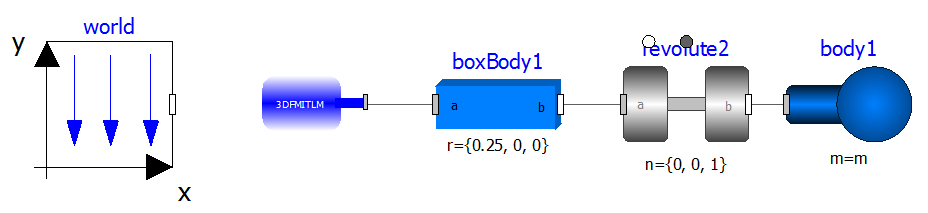
\includegraphics[width=0.85\textwidth]{figs/model_omedit.png}
\caption{The second half of the first beam and the second beam  are modelled in OpenModelica}
\label{fig:model_omedit}
\end{figure}

\subsection{Building co-simulation system model}

When both FMUs have been generated together with one \texttt{fmi.config} file each, it is time to build the meta model.
\begin{enumerate}
\item \textbf{Create a new meta model.}\\
             Either by hand or by using the graphical user interface.
\item \textbf{Add the FMUs as sub-models.}\\
              Use \texttt{StartTLMFmiWrapper} as start command.
\item \textbf{Fetch TLM interfaces.}
\item \textbf{Add a connection between the two models.}\\
              Default TLM parameters should work fine.
\item \textbf{Make sure interfaces are aligned.}
\item \textbf{Choose solver for model exchange.}\\
              By editing \texttt{StartTLMFmiWrapper.bat}.\\
              Use for example \texttt{solver=CVODE} or \texttt{solver=IDA}.
\end{enumerate}

When done, the meta model XML file should look similar to listing \ref{lst:metamodel_xml}.
In the graphical interface, the meta model should look like figure \ref{fig:metamodel_omedit}.
The model is now ready to be simulated!

\begin{lstlisting}[language=xml,float,floatplacement=ht,label={lst:metamodel_xml},caption=XML description of the complete meta model]
<?xml version='1.0' encoding='ISO-8859-1'?>
<Model Name="doublePendulum">
  <SubModels>
    <SubModel Name="doublePendulum1" 
              ModelFile="doublePendulum1.fmu"
              StartCommand="StartTLMFmiWrapper" 
              Position="0,0,0" 
              Angle321="0,0,0">
      <InterfacePoint Name="tlm" 
                      Position="0.25,0,0" 
                      Angle321="0,0,0"/>
    </SubModel>
    <SubModel Name="doublePendulum2" 
              ModelFile="doublePendulum2.fmu" 
              StartCommand="StartTLMFmiWrapper" 
              Position="0.25,0,0"  
              Angle321="0,0,0">
      <InterfacePoint Name="tlm" 
                      Position="0,0,0" 
                      Angle321="0,0,0"/>
    </SubModel>
  </SubModels>
  <Connections>
    <Connection From="doublePendulum1.tlm" 
                To="doublePendulum2.tlm" 
                Delay="1e-4" 
                Zf="10000"   
                Zfr="100"
                alpha="0.2">
    </Connection>
  </Connections>
  <SimulationParams ManagerPort="11113" StopTime="3" StartTime="0"/>
</Model>
\end{lstlisting}

\begin{figure}[ht]
\centering
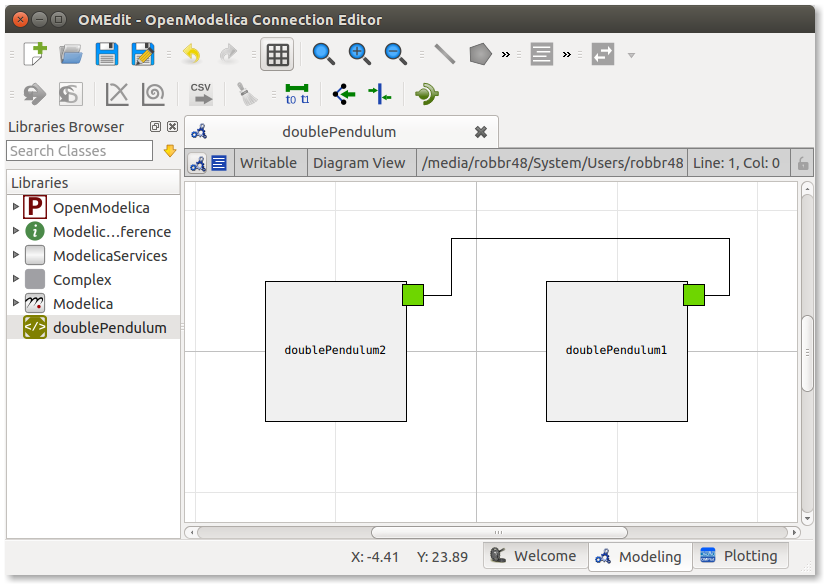
\includegraphics[width=0.75\textwidth]{figs/metamodel.png}
\caption{Graphical view of the complete meta model}
\label{fig:metamodel_omedit}
\end{figure}